\section{Results}\label{sec:results}

In this section, we present our experimental outcomes from fine-tuning BERT on the Civil Comments dataset and discuss how various hyperparameters affect both model performance and computational efficiency. We highlight key insights gleaned from different configurations, explain their implications for deployment, and compare our findings to established practices in the literature.

\subsection{Findings}

Our experimental results indicate that BERT outperforms baseline models across all examined metrics, as shown in \cref{tab:bert_performance}. This demonstrates the effectiveness of BERT in handling the complexities of the Civil Comments dataset and highlights its superior performance in toxic comment classification tasks.

\begin{table}[h!]
    \centering
    \caption{BERT performance on the Civil Comments test dataset}
    \label{tab:bert_performance}
    \resizebox{\textwidth}{!}{%
    \begin{tabular}{lcccccccc}
    \hline
    \textbf{Precision (C1)} & \textbf{Recall (C1)} & \textbf{F1 (C1)} & \textbf{Macro F1} & \textbf{Weighted F1} & \textbf{Acc.} & \textbf{AUC ROC} & \textbf{Loss} \\ \hline
    0.67 & 0.75 & 0.70 & 0.84 & 0.96 & 0.96 & 0.9731 & 0.2317 \\ \hline
    \end{tabular}%
    }
\end{table}

\noindent Our experiments revealed several key insights into the impact of hyperparameters on model performance and computational efficiency. These findings are summarized below:

\paragraph{Sequence length:} Reducing the sequence length to 128 tokens achieved a 4x speed-up in training time. As illustrated in \cref{fig:seq_len}, while comments in the validation dataset can be up to 256 tokens, the majority of comments fall well within 128 tokens. This reduction had no significant impact on model performance, suggesting that 128 tokens are sufficient for capturing the essential context of most comments.

\begin{figure}[ht]
    \centering
    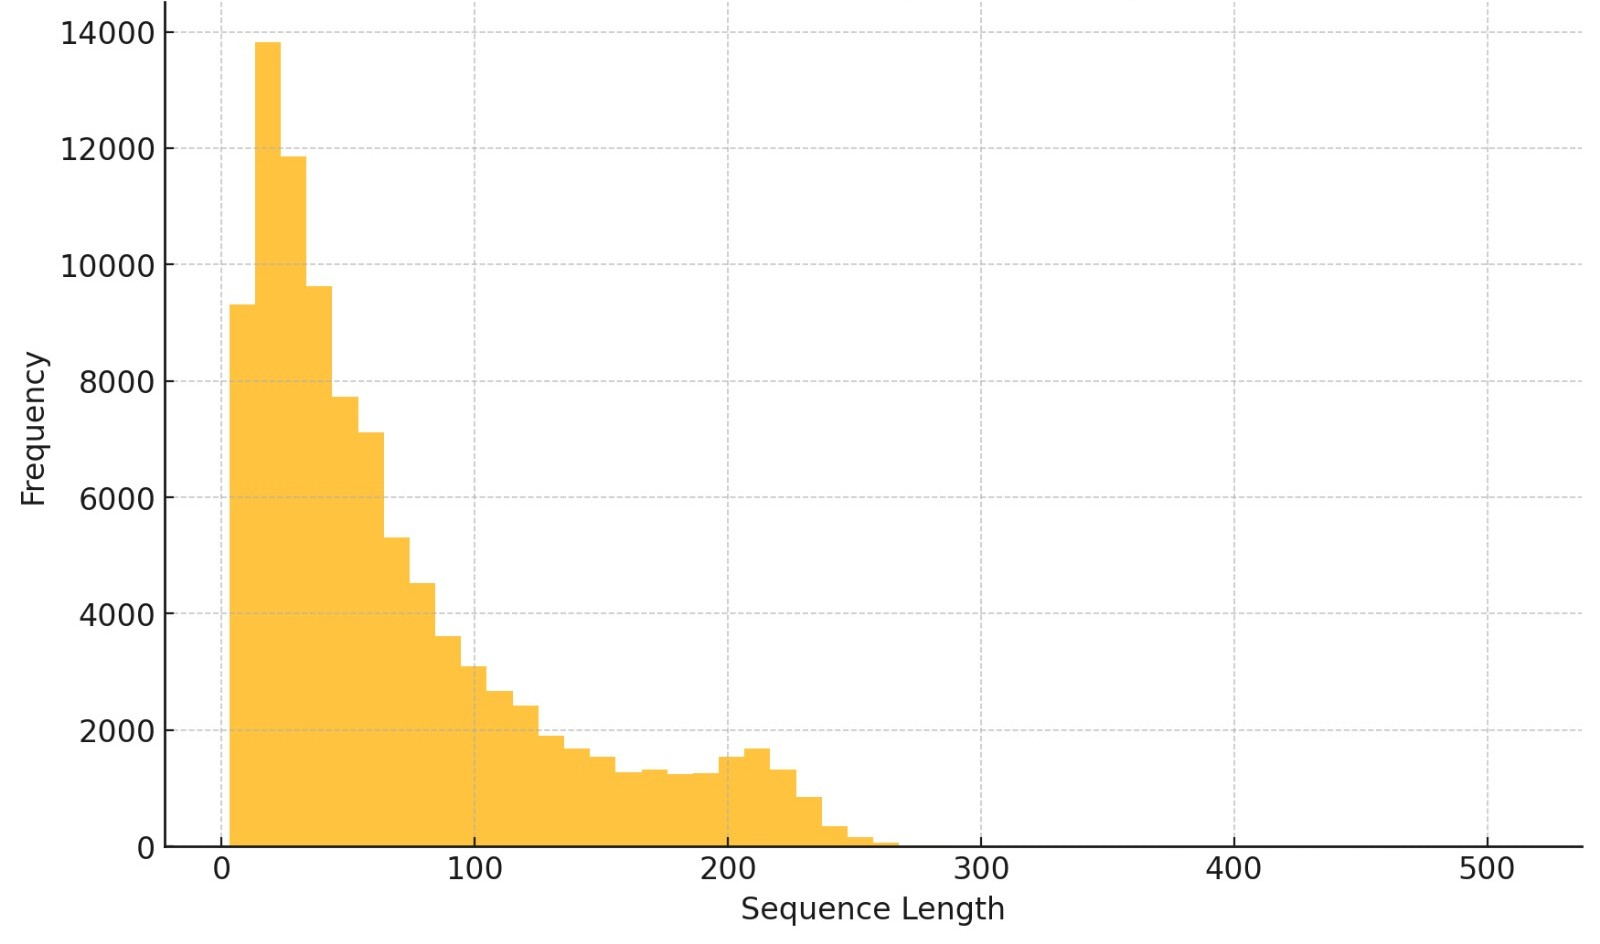
\includegraphics[width=0.7\textwidth]{./figures/seq_len.jpg}
    \caption{Distribution of comment lengths in the Civil Comments validation dataset.}
    \label{fig:seq_len}
\end{figure}

\paragraph{Positive proportion:} A positive class proportion of \texttt{pos\_proportion=0.1} showed no significant impact on the model's performance, with changes in metrics remaining negligible (\(\leq 1\%\)). Despite this minimal effect on performance, this configuration achieved a substantial 38\% reduction in data processing time. This outcome suggests that \texttt{pos\_proportion=0.1} offers an optimal balance between computational efficiency and model effectiveness, making it particularly suitable for scenarios constrained by limited computational resources.

\paragraph{Batch size:} Fine-tuning with larger batch sizes consistently yielded similar model performance while slightly increasing speed (17\% faster). The maximum batch size that fits into the available GPU memory was 1024, which further highlights the efficient utilization of resources during fine-tuning.

\paragraph{Preprocessing:} Applying preprocessing techniques had no discernible positive impact on model performance. This suggests that the model's tokenizer and pre-trained embeddings are sufficiently robust to handle raw input data without additional preprocessing steps.

\paragraph{Learning rate:} A grid search across learning rates \([10^{-7}, 10^{-6}, 10^{-5}, 10^{-4}, 10^{-3}]\) revealed that values within the range \([10^{-6}, 10^{-5}, 10^{-4}]\) were most effective. In contrast, both extremely low and extremely high learning rates prevented the model from effectively learning to identify the toxic class, leading to convergence failure or instability. These results underscore the necessity of selecting an intermediate learning rate to ensure stable and reliable training.

\paragraph{Number of epochs:} Extending training beyond the first epoch did not result in improved model performance. For example, even with five epochs and a weight decay of 1.0, no notable gains were observed. While training for multiple epochs we also tried employing a cosine annealing schedule to adjust the learning rate, this did not lead to improvements in the validation metrics.

\paragraph{Weight decay:} Applying weight decay had no meaningful effect on the model's performance. Only excessively high values led to a noticeable reduction in the model's learning capacity, reinforcing the importance of choosing reasonable values for this hyperparameter.

\subsection{Comparison to literature}

Several of the chosen hyperparameters align with established practices in the literature. For example, setting the sequence length to 128 tokens (or even less) is a common strategy to balance computational efficiency with model performance. \cite{Zhao2021}

For batch size, larger values like 1024 are feasible on modern GPUs and are known to improve training speed without adversely affecting generalization. Similarly, the chosen learning rate of \(1e^{-4}\) falls within the range of other researchers, who fine-tuned BERT for various NLP tasks. \cite{Smith2017, Zhou2021}

The decision to avoid preprocessing is supported by Kurniasih et al., who highlight that advancements in modern tokenization methods significantly reduce the necessity for extensive input cleaning, enabling models to effectively handle raw text data without substantial preprocessing efforts. \cite{Kurniasih2022}

The decision to use only a single epoch for fine-tuning is informed by the reduced need for extensive training in larger pre-trained models, where early stopping can still yield strong generalization performance. Similarly, the impact of weight decay appears to be less critical, as other regularization techniques, such as dropout, are already applied. \cite{Kundu2023,vaswani2017attention}


\subsection{Chosen configuration}\label{subsec:chosen_configuration}
In summary, the fine-tuning of BERT for toxic comment classification demonstrates the importance of judicious hyperparameter selection. Reducing sequence length to 128 tokens resulted in substantial computational gains with no loss in performance. Larger batch sizes were utilized effectively, balancing memory constraints and training speed. Weight decay and preprocessing were found to have minimal impact while learning rates within \([10^{-6},10^{-5}, 10^{-4}]\) proved optimal for convergence. Additionally, extending training beyond one epoch provided no significant advantages, confirming the sufficiency of shorter training durations. Leveraging an 8x NVIDIA A100 80~GB GPU setup, the model achieved fine-tuning plus evaluation within an impressive seven minutes. 

\noindent The chosen hyperparameter configuration is as follows:

\[
\text{Config}\left(
\begin{aligned}
    &\text{sequence\_len} = 128, \\
    &\text{pos\_proportion} = 0.1, \\
    &\text{batch\_size} = 1024, \\
    &\text{preprocessing} = \text{False}, \\
    &\text{learning\_rate} = 1e-4, \\
    &\text{num\_epochs} = 1, \\
    &\text{weight\_decay} = 0, \\
    &\text{optimizer} = \text{AdamW}, \\
    &\text{loss} = \text{BCEWithLogitsLoss}
\end{aligned}
\right)
\]

\noindent This setup provides a robust balance between computational efficiency and model performance, forming a strong foundation for scalable real-world deployment.


